\PassOptionsToPackage{subsection=false}{beamerouterthememiniframes}
\PassOptionsToPackage{dvipsnames,table}{xcolor}
\documentclass[fleqn]{beamer}
\usepackage{graphicx}
\usepackage{multirow}
\usepackage{multicol}
\usepackage{amsmath,amsfonts,amsthm,amsopn}
\usepackage{color, colortbl}
\usepackage{subfig}
\usepackage{wrapfig}
\usepackage{fancybox}
\usepackage{tikz}
\usepackage{fancyhdr}
\usepackage{setspace}
\usepackage{xcolor}
\usepackage{movie15}
\usepackage{pifont}
\usepackage{soul}
\usepackage{fancyvrb,newverbs}
\usepackage{epsfig}
\usepackage{epstopdf}
\fvset{fontsize=\footnotesize}
\RecustomVerbatimEnvironment{verbatim}{Verbatim}{}

%\usepackage{fancybox}

\usetheme{Szeged}
\usecolortheme{default}

%\definecolor{links}{HTML}{2A1B81}
%\definecolor{links}{blue!20}
\hypersetup{colorlinks,linkcolor=,urlcolor=blue!80}

\setbeamertemplate{blocks}[rounded]
\setbeamercolor{block title}{bg=blue!40,fg=black}
\setbeamercolor{block body}{bg=blue!10}


\newenvironment<>{clicker}[1]{%
  \begin{actionenv}#2%
      \def\insertblocktitle{#1}%
      \par%
      \mode<presentation>{%
        \setbeamercolor{block title}{fg=white,bg=magenta}
       \setbeamercolor{block body}{fg=black,bg=magenta!10}
       \setbeamercolor{itemize item}{fg=magenta}
       \setbeamertemplate{itemize item}[triangle]
       \setbeamercolor{enumerate item}{fg=magenta}
     }%
      \usebeamertemplate{block begin}}
    {\par\usebeamertemplate{block end}\end{actionenv}}

%\newcommand{\bmp}{\begin{minipage}}
%\newcommand{\emp}{\end{minipage}}
%\newcommand{\blankcolumn}{\bmp{.05\textwidth}\hspace{0.50in} \emp}

\defbeamertemplate*{footline}{infolines theme}
{
  \leavevmode%
  \hbox{%
  \begin{beamercolorbox}[wd=.333333\paperwidth,ht=2.25ex,dp=1ex,left]{author in head/foot}%
    \usebeamerfont{author in head/foot}~~\insertshortinstitute: \insertshorttitle
  \end{beamercolorbox}%
  \begin{beamercolorbox}[wd=.67\paperwidth,ht=2.25ex,dp=1ex,right]{date in head/foot}%
    \usebeamerfont{date in head/foot}%\insertshortdate{}\hspace*{2em}
    \insertframenumber{} / \inserttotalframenumber\hspace*{2ex}
  \end{beamercolorbox}
  }%
  \vskip0pt%
}

\newcommand{\cmark}{\ding{51}}%
\newcommand{\xmark}{\ding{55}}%
\newcommand{\grp}{\textcolor{magenta}{Group Exercise}}
\newcommand{\grpc}{\textcolor{magenta}{Group Exercise, continued}}
\newcommand{\bsans}[1]{\underline{\hspace{0.2in}\color{blue!80}{#1}\hspace{0.2in}}}

\definecolor{cverbbg}{gray}{0.93}
\newenvironment{cverbatim}
 {\SaveVerbatim{cverb}}
 {\endSaveVerbatim
  \flushleft\fboxrule=0pt\fboxsep=.5em
  \colorbox{cverbbg}{\BUseVerbatim{cverb}}%
  \endflushleft
}
\newenvironment{lcverbatim}
 {\SaveVerbatim{cverb}}
 {\endSaveVerbatim
  \flushleft\fboxrule=0pt\fboxsep=.5em
  \colorbox{cverbbg}{%
    \makebox[\dimexpr\linewidth-2\fboxsep][l]{\BUseVerbatim{cverb}}%
  }
  \endflushleft
}

\newcommand{\bmp}{\begin{minipage}}
\newcommand{\emp}{\end{minipage}}
\newcommand{\blankcolumn}{\bmp{.05\textwidth}\hspace{0.50in} \emp}

 \newenvironment{code}[1]%
  {\vspace{.1in}\footnotesize\Verbatim[frame=single,label=SAS Code,commandchars=\\\{\},xrightmargin=#1\textwidth,framesep=.2in,labelposition=all]}
  {\endVerbatim\normalsize}

 \newenvironment{Rcode}[1]%
  {\vspace{.1in}\footnotesize\Verbatim[frame=single,label=R Code,commandchars=\\\{\},xrightmargin=#1\textwidth,framesep=.2in,labelposition=all]}
  {\endVerbatim\normalsize}

   \newenvironment{RcodeScript}[1]%
  {\vspace{.1in}\scriptsize\Verbatim[frame=single,label=R Code,commandchars=\\\{\},xrightmargin=#1\textwidth,framesep=.2in,labelposition=all]}
  {\endVerbatim\normalsize}

 \newenvironment{RcodeTiny}[1]%
  {\vspace{.1in}\tiny\Verbatim[frame=single,label=R Code,commandchars=\\\{\},xrightmargin=#1\textwidth,framesep=.2in,labelposition=all]}
  {\endVerbatim\normalsize}


   \newenvironment{Rout}[1]%
  {\vspace{.1in}\footnotesize\Verbatim[frame=single,label=R Output,commandchars=\\\{\},xrightmargin=#1\textwidth,framesep=.2in,labelposition=all]}
  {\endVerbatim\normalsize}
  
     \newenvironment{MTout}[1]%
  {\vspace{.1in}\footnotesize\Verbatim[frame=single,label=Minitab Output,commandchars=\\\{\},xrightmargin=#1\textwidth,framesep=.2in,labelposition=all]}
  {\endVerbatim\normalsize}

   \newenvironment{RoutScript}[1]%
  {\vspace{.1in}\scriptsize\Verbatim[frame=single,label=R Output,commandchars=\\\{\},xrightmargin=#1\textwidth,framesep=.2in,labelposition=all]}
  {\endVerbatim\normalsize}

 \newenvironment{RoutTiny}[1]%
  {\vspace{.1in}\tiny\Verbatim[frame=single,label=R Output,commandchars=\\\{\},xrightmargin=#1\textwidth,framesep=.2in,labelposition=all]}
  {\endVerbatim\normalsize}

\newenvironment{craw}[2]%
{\vspace{.1in}\footnotesize\Verbatim[frame=single,label=#2,commandchars=\\\{\},xrightmargin=#1\textwidth,framesep=.2in,labelposition=all]}
  {\endVerbatim\normalsize}


\newenvironment{scriptcraw}[2]%
{\vspace{.1in}\scriptsize \Verbatim[frame=single,label=#2,commandchars=\\\{\},xrightmargin=#1\textwidth,framesep=.2in,labelposition=all]}
  {\endVerbatim\normalsize}

  \newenvironment{tinycraw}[2]%
{\vspace{.1in}\tiny \Verbatim[frame=single,label=#2,commandchars=\\\{\},xrightmargin=#1\textwidth,framesep=.2in,labelposition=all]}
  {\endVerbatim\normalsize}




\title[Set 11]{Cox regression models with multiple predictors:\\ interactions, comparing models, model diagnostics}
\author[Pileggi]{Shannon Pileggi}

\institute[STAT 417]{STAT 417}

\date{}


\begin{document}

\begin{frame}
\titlepage
\end{frame}

\begin{frame}
\frametitle{OUTLINE\qquad\qquad\qquad} \tableofcontents[hideallsubsections]
\end{frame}


%===========================================================================================================================
\section[Interactions]{Interactions}
%===========================================================================================================================
\subsection{}

\begin{frame}
\frametitle{Visualizing interactions}
Recall the VALCG lung cancer study.  Suppose we believe that the standard treatment is more effective than the test treatment for patients with lower Karnofsky scores, but less effective than the test treatment for patients with higher Karnofsky scores.  Create a plausible sketch of this scenario.\\
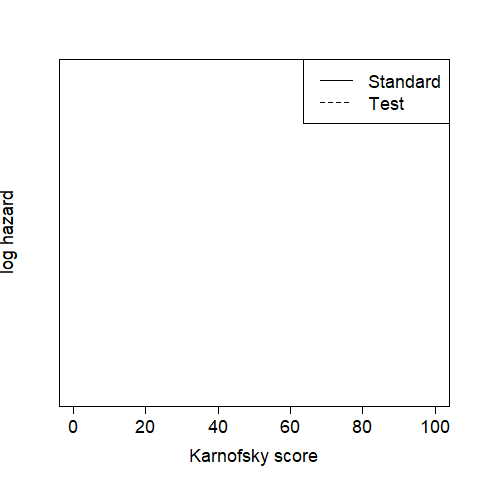
\includegraphics[width=0.5\textwidth]{Figures/blank_interaction.png}
\end{frame}

\begin{frame}
\frametitle{Interactions}
What does an interaction between $X_1$ and $X_2$ imply?
\vskip70pt
%the effect of $X_1$ on the hazard rate (at any time $t$) depends on the level of the second predictor $X_2$
When an interaction exists:
\begin{enumerate}
\item Include both $X_1$ and $X_2$ in the model (main effects).
\item In addition, include \emph{interaction terms}:
\item[]
\end{enumerate}
\begin{tabular}{lll}
\hline
$X_1$ & $X_2$ & Interaction term(s) \\
\hline\hline
quant. & quant & $X_1X_2$ \\
quant & cat. ($k$)   & $X_1D_1, X_1D_2,.. X_1D_{k-1}$ \\
cat. ($j$)  & cat. ($k$)  & $(j-1)(k-1)$ products of dummy variables \\
\hline
\end{tabular}
\end{frame}


\begin{frame}
\frametitle{Discussion}
Suppose we are using a Cox regression model for the hazard of lung cancer with the variables $X_1=$ Karnofsky score, $X_2=$ treatment (where $X_2=0$ for standard, and $X_2=1$ for test treatment), and the interaction between $X_1$ and $X_2$.
\begin{clicker}{How many \emph{parameters} are estimated for this model?}
\begin{enumerate}
\item[1]
\item[2]
\item[3]
\item[4]
\item[5]
\end{enumerate}
\end{clicker}
Write out the model:
\vskip100pt
\end{frame}


\begin{frame}[fragile]
\frametitle{Interactions in \texttt{R}}
In \texttt{R} model formula syntax:
\begin{itemize}
\item[\fbox{\texttt{:}}] indicates interaction
\item[\fbox{\texttt{*}}] indicates main effects plus interaction
\item[]
\end{itemize}
The following two model specifications are \emph{equivalent}:
\begin{Rcode}{-0.03}
CR_mod1 <- coxph(Surv(time, status) ~ karno + trt + karno:trt,
                data = veteran)

CR_mod2 <- coxph(Surv(time, status) ~ karno*trt,
                data = veteran)
\end{Rcode}
\end{frame}

\begin{frame}[fragile]
\frametitle{\texttt{R} output}
\begin{Rout}{0.0}
Call:
coxph(formula = Surv(time, status) ~ karno * trt, data = veteran)

  n= 137, number of events= 128

               coef exp(coef)  se(coef)      z Pr(>|z|)
karno     -0.008668  0.991369  0.016704 -0.519   0.6038
trt        1.093251  2.983959  0.606419  1.803   0.0714 .
karno:trt -0.015867  0.984258  0.009954 -1.594   0.1109
---
Signif. codes:  0 ‘***’ 0.001 ‘**’ 0.01 ‘*’ 0.05 ‘.’ 0.1 ‘ ’ 1

          exp(coef) exp(-coef) lower .95 upper .95
karno        0.9914     1.0087    0.9594     1.024
trt          2.9840     0.3351    0.9091     9.794
karno:trt    0.9843     1.0160    0.9652     1.004
\end{Rout}
\end{frame}

\begin{frame}
\frametitle{Understanding the interaction}
\begin{itemize}
\item Estimate the hazard ratio corresponding to a 10 point increase in Karnofsky score for those on the \emph{standard} treatment.
\item[]
\item[]
\item[]
\item[]
\item[]
\item Estimate the hazard ratio corresponding to a 10 point increase in Karnofsky score for those on the \emph{test} treatment.
\item[]
\item[]
\item[]
\item[]
\item[]
\item What does this mean?
\item[]
\item[]
\item[]
\end{itemize}
\end{frame}

\begin{frame}[fragile]
\frametitle{Assessing significance of the interaction}
\begin{Rout}{0.0}
               coef exp(coef)  se(coef)      z Pr(>|z|)
karno     -0.008668  0.991369  0.016704 -0.519   0.6038
trt        1.093251  2.983959  0.606419  1.803   0.0714
karno:trt -0.015867  0.984258  0.009954 -1.594   0.1109
...
Likelihood ratio test= 45.52  on 3 df,   p=7.173e-10
Wald test            = 49.11  on 3 df,   p=1.238e-10
Score (logrank) test = 51.39  on 3 df,   p=4.04e-11
\end{Rout}
Is there evidence that the association between hazard and Karnofsky score depends on treatment?
\vskip200pt
\end{frame}

%===========================================================================================================================
\section[Nested models]{Comparing nested models}
%===========================================================================================================================
\subsection{}
\begin{frame}
\tableofcontents[currentsection, hideallsubsections]
\end{frame}

\begin{frame}
\frametitle{Model selection}
\begin{itemize}
\item There are many strategies to select a final set of predictors.
%\item[]
\item One method is to compare \emph{nested} models:
\begin{itemize}
\item The \textbf{full model} contains the predictors $X_1,X_2,\ldots,X_f$.
\item The \textbf{reduced model} contains a subset of those predictors, say $r$ out of the $f$ predictors where $r < f$.
\end{itemize}
%\item[]
\item For formal comparison of nested models, use the partial likelihood ratio test by comparing the evaluated log partial likelihood functions of the full and reduced models.
%\item[]
\item This allows us to determine if the inclusion of additional predictors into a model can ``improve" the model, i.e. the goodness-of-fit is significantly improved.
\end{itemize}
\end{frame}

\begin{frame}
\frametitle{VALCG lung cancer potential predictors}
\begin{tabular}{r|c|l}
\texttt{karno} & $X_1$ & Karnofsky score (100=good; 0=dead); \\
               & &(measures cancer patients' functional impairment) \\
& \\
\texttt{trt} & $X_2$ & Treatment type (0=standard, 1=test) \\
& \\
\texttt{celltype} & $X_3$& cancer cell type (squamous, smallcell, adeno, large) \\
& \\
\texttt{age} & $X_4$ & patients age in years at time of treatment start \\
& \\
\texttt{diagtime} & $X_5$ & months from diagnosis to treatment assignment \\
& \\
\texttt{prior} & $X_6$ & prior therapy to the treatment (0=no, 1=yes) \\
\end{tabular}
\end{frame}

\begin{frame}
\frametitle{Discussion}
Consider the following model which contains:\\
\vskip10pt
\textbf{Model 0:} \texttt{celltype}, \texttt{age}, \texttt{trt}, and \texttt{celltype}$\times$\texttt{trt}
\vskip20pt
\begin{clicker}{Which of the following models would be nested in \textbf{Model 0}?}
\begin{enumerate}
\item[Model 1:] \texttt{celltype}, \texttt{age}, \texttt{karno}
\item[Model 2:] \texttt{age}, \texttt{trt}
\item[Model 3:] \texttt{celltype}, \texttt{trt}, and \texttt{celltype}$\times$\texttt{trt}
\item[Model 4:] \texttt{celltype}, \texttt{age}, \texttt{trt}, \texttt{prior}
\end{enumerate}
\end{clicker}
\end{frame}


\begin{frame}
\frametitle{Discussion}

\begin{itemize}
\item[\textbf{Model 1}:] \texttt{karno}, \texttt{trt}, \texttt{celltype}, \texttt{age}, \texttt{karno}$\times$\texttt{age}, \texttt{karno}$\times$\texttt{celltype}
\item[]
\item[\textbf{Model 2}:] \texttt{karno}, \texttt{trt}, \texttt{celltype}, \texttt{age}
\item[]
\end{itemize}
\begin{clicker}{How many parameters will be estimated in}
\begin{enumerate}
\item[] Model 1?
\item[] Model 2?
\end{enumerate}
\end{clicker}
Determine if the regression model improves fit with the addition of the interaction terms.
\begin{itemize}
\item[$H_0$:]
\item[]
\item[$H_a$:]
\item[]
\end{itemize}
\end{frame}


\begin{frame}
\frametitle{Partial likelihood ratio test}
\begin{itemize}
\item[$f=$]
\item[]
\item[$r=$]
\item[]
\item[$l_f=$]
\item[]
\item[$l_r=$]
\item[]
\item[$df=$]
\item[]
\item[$G_l=$]
\item[]
\end{itemize}
\end{frame}

\begin{frame}[fragile]
\frametitle{Create the models}
\hspace*{-0.3in}
\begin{Rcode}{-0.05}
CR_full <-
    coxph(Surv(time, status) ~ karno + trt + celltype + age +
                               karno:age + karno:celltype,
            data = veteran)

CR_red <-
    coxph(Surv(time, status) ~ karno + trt + celltype + age,
            data = veteran)
\end{Rcode}
\end{frame}

\begin{frame}[fragile]
\frametitle{Full model}
\hspace*{-0.3in}
\begin{Rout}{-0.05}
                              coef  exp(coef)   se(coef)      z Pr(>|z|)
karno                   -0.1135446  0.8926644  0.0366088 -3.102  0.00193 **
trt                      0.2824701  1.3264021  0.2081975  1.357  0.17486
celltypelarge           -1.5886004  0.2042112  1.1776847 -1.349  0.17736
celltypesmallcell       -1.4601698  0.2321968  0.8357294 -1.747  0.08061 .
celltypesquamous        -0.9505561  0.3865260  0.9233413 -1.029  0.30326
age                     -0.0769218  0.9259623  0.0313400 -2.454  0.01411 *
karno:age                0.0012390  1.0012398  0.0005325  2.327  0.01999 *
karno:celltypelarge      0.0095336  1.0095792  0.0178371  0.534  0.59301
karno:celltypesmallcell  0.0179957  1.0181586  0.0138276  1.301  0.19311
karno:celltypesquamous  -0.0069418  0.9930822  0.0150711 -0.461  0.64508
\end{Rout}
\end{frame}

\begin{frame}[fragile]
\frametitle{Reduced model}
\hspace*{-0.3in}
\begin{Rout}{-0.05}
                       coef exp(coef)  se(coef)      z Pr(>|z|)
karno             -0.032685  0.967843  0.005409 -6.043 1.51e-09 ***
trt                0.303048  1.353980  0.205656  1.474   0.1406
celltypelarge     -0.776475  0.460025  0.297703 -2.608   0.0091 **
celltypesmallcell -0.322467  0.724360  0.268923 -1.199   0.2305
celltypesquamous  -1.178807  0.307646  0.296440 -3.977 6.99e-05 ***
age               -0.008903  0.991136  0.009224 -0.965   0.3345
\end{Rout}
\end{frame}

\begin{frame}[fragile]
\frametitle{Computing the test statistic}
\begin{minipage}{0.5\textwidth}
\begin{Rout}{0.0}
> CR_full$loglik
[1] -505.4491 -469.9852

> CR_red$loglik
[1] -505.4491 -474.4578
\end{Rout}
\begin{clicker}{Match the following values to:\\ $l_p(0)$, $l_f$, $l_r$.}
\begin{enumerate}
\item -505.4491
\item -469.9852
\item -474.4578
\end{enumerate}
\end{clicker}
\end{minipage}
\blankcolumn
\begin{minipage}{0.4\textwidth}
\begin{enumerate}
\item Calculate the partial likelihood ratio test statistic.
\item[]
\item[]
\item[]
\item[]
\item[]
\item[]
\item What is the degrees of freedom?
\item[]
\item[]
\item[]
\item[]
\end{enumerate}
\end{minipage}
\end{frame}

\begin{frame}[fragile]
\frametitle{Computing the $p$-value and conclusion}
\begin{Rcode}{.25}
pchisq(q = 8.945, df = 4, lower.tail = F)
\end{Rcode}
\begin{Rout}{.25}
0.06248902
\end{Rout}
What does this suggest about the inclusion of interaction terms in the model?
\vskip200pt
\end{frame}

%===========================================================================================================================
\section[Non-nested models]{Comparing non-nested models}
%===========================================================================================================================
\subsection{}
\begin{frame}
\tableofcontents[currentsection, hideallsubsections]
\end{frame}

\begin{frame}
\frametitle{AIC for non-tested models}
\begin{itemize}
\item We can use Akaike's Information Criterion (AIC) to compare non-nested models
\item[]
\item[] $AIC = -2l_p(\hat{\beta})+2p$
\item[]
\item The \emph{smaller} the value of AIC, the \emph{better} the fit of the current model to the data.
\item There is no formal inference procedure to compare AIC values for different models.
\item Some subjective judgment must be used to determine if a model with a slightly smaller value of AIC is better.
\end{itemize}
\end{frame}

\begin{frame}[fragile]
\frametitle{Comparing non-nested models}
\begin{Rcode}{0.0}
CR_mod1 <- coxph(Surv(time, status) ~ karno + celltype,
                 data = veteran)

CR_mod2 <- coxph(Surv(time, status) ~ trt + celltype + age,
                data = veteran)
\end{Rcode}
\begin{minipage}{0.45\textwidth}
\begin{Rout}{0.0}
> CR_mod1$loglik
[1] -505.4491 -475.7632

> CR_mod2$loglik
[1] -505.4491 -492.4281
\end{Rout}
\end{minipage}
\blankcolumn
\begin{minipage}{0.45\textwidth}
\begin{enumerate}
\item[M1:] AIC =
\item[]
\item[]
\item[M2:] AIC =
\item[]
\item[]
\end{enumerate}
\end{minipage}
\end{frame}



%===========================================================================================================================
\section[Adjusted $\hat{S}$(t)]{Adjusted $\hat{S}(t)$}
%===========================================================================================================================
\subsection{}
\begin{frame}
\tableofcontents[currentsection, hideallsubsections]
\end{frame}

\begin{frame}
\frametitle{The idea}
\begin{itemize}
\item We can compute \emph{predicted survival curves} for \emph{fixed} values of explanatory variables.
\item The CR model is given by:
\item[] \hspace{0.3in} $h(t|X_1,\ldots,X_p)= h_0(t)\exp(\beta_1X_1+\cdots+\beta_pX_p)$
\item The cumulative hazard function at time $t$ given $X_1,\ldots,X_p$:
\item[]\hspace{0.3in}  $H(t|X_1,\ldots,X_p)$
\item The survival function at time $t$ given $X_1,\ldots,X_p$:
\item[]\hspace{0.3in}  $S(t|X_1,\ldots,X_p)$
\item Putting it together:
\item[] \hspace{0.3in}  $S(t) = e^{-H(t)}$
\end{itemize}
\end{frame}

\begin{frame}
\frametitle{Predictor-adjusted survival probabilities}
\begin{eqnarray*}
% \nonumber % Remove numbering (before each equation)
  S(t|X_1,\ldots,X_p) &=& e^{H(t|X_1,\ldots,X_p)} \\
    &=& e^{-\int_0^t h(y|X_1,\ldots,X_p)dy} \\
    &=& e^{-\int_0^t h_0(y)\exp\left(\sum\limits_{j=1}^{p}\beta_jX_j\right)dy}  \\
    &=& \left[e^{-\int_0^t h_0(y)dy}\right]^{\exp\left(\sum\limits_{j=1}^{p}\beta_jX_j\right)} \\
    &=& \left[S_0(t)\right]^{\exp\left(\sum\limits_{j=1}^{p}\beta_jX_j\right)}\\
    & & \\
  \hat{S}(t|X_1,\ldots,X_p) &=&  \left[\hat{S}_0(t)\right]^{\exp\left(\sum\limits_{j=1}^{p}\hat{\beta}_jX_j\right)}\\
\end{eqnarray*}
\end{frame}


\begin{frame}[fragile]
\frametitle{Lung cancer example}
Estimate the survival probabilities for lung cancer patients with Karnofsky scores of 10 and 90.
\begin{Rcode}{0.0}
KM_obj <- survfit(Surv(time, status) ~ 1,
                  conf.type = "none",
                  data = veteran)

CR_mod <- coxph(Surv(time, status) ~ karno, data = veteran)

pred_max_karno <- data.frame(karno = 90, veteran)
pred_min_karno <- data.frame(karno = 10, veteran)

adj_surv_max <- survfit(CR_mod, newdata = pred_max_karno)
adj_surv_min <- survfit(CR_mod, newdata = pred_min_karno)
\end{Rcode}
\end{frame}


\begin{frame}[fragile]
\frametitle{Adjusted survival curves}
\hspace*{-0.3in}
\begin{minipage}{0.58\textwidth}
\begin{Rcode}{0.0}
plot(KM_obj,
     xlab = "Days",
     ylab = "Est. survival prob.")
lines(adj_surv_min, lty = 2)
lines(adj_surv_max, lty = 3)
legend("topright",
       c("Unadjusted",
         "Karno = 10",
         "Karno = 90"),
       lty = 1:3)
\end{Rcode}
\end{minipage}
%\blankcolumn
\begin{minipage}{0.42\textwidth}
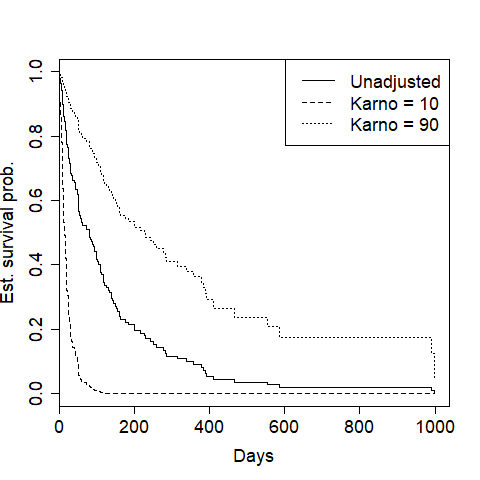
\includegraphics[width=1.0\textwidth]{Figures/karno_adj.png}
\end{minipage}
\end{frame}


%===========================================================================================================================
\section[Model assessment]{Model assessment}
%===========================================================================================================================
\subsection{}
\begin{frame}
\tableofcontents[currentsection, hideallsubsections]
\end{frame}

\begin{frame}
\frametitle{Model assumptions and other checks}
Assumptions to assess:
\begin{itemize}
\item \textit{Proportional hazards}: the effect of the predictors on hazard does not depend on (vary by) time:
\item[]
\item[]
\item[]
\item \textit{Effect of each predictor on log hazard is linear}:
\item[]
\item[]
\item[]
\end{itemize}

Other checks:
\begin{itemize}
\item \textit{Outliers}, i.e. identify subjects whose outcome is poorly predicted by the CR model.
\item \textit{Influential subjects}, i.e. individuals with ``unusual" values for a specific predictor.
%(analogous to screening for individuals with high leverage).
\end{itemize}
\end{frame}

\begin{frame}
\frametitle{Residuals}
\begin{itemize}
\item Recall from linear regression \textit{residuals} are used to check key model assumptions and evaluate model adequacy.
\item For linear models, the residual for the $i^{th}$ subject is:
\begin{eqnarray}
e_i=y_i-\hat{y}_i\nonumber
\end{eqnarray}
%where $y_i$ is the observed value of the response variable and $\hat{y}_i$ the predicted value of $y$ at the value of the predictor $x_i$.
%\item We have discussed model-based inferences and interpretations under the assumption that the hazards
%are proportional.
\item There is no exact analog to this definition when using the CR model, but there are several ``developed" types of residuals that can be used for checking different aspects of model adequacy:
\begin{itemize}
\item Martingale residuals %Assessing the adequacy of the functional form of a predictor, or determining what the functional form should be.
\item Deviance residuals % check for outliers, i.e. identify individuals whose outcome is poorly predicted
\item Schoenfeld residuals %useful for identifying violations of the proportional hazards assumption
\item Score residuals %detecting overly influential observations.
\end{itemize}
\end{itemize}
\end{frame}


\begin{frame}
\frametitle{Martingale residuals}
\hspace*{-0.3in}
\begin{minipage}{0.12\textwidth}
\textcolor{white}{w}
\end{minipage}
\begin{minipage}{0.91\textwidth}
\small{
\begin{itemize}
\item[Use] Assessing the adequacy of the functional form of a predictor, or determining what the functional form should be.
\item[Definition] Difference between the \textit{observed} number of events experienced by subject $i$ and the \textit{expected} number of events experienced by subject $i$ (under
the current model).
\item[Applies to] All subjects, for each predictor
\item[Interpretation] $>0$: subject $i$ experienced the event earlier than expected \\
                      $<0$: subject $i$ experienced the event later than expected
\item[Result] vector of length $n$ (\# of subjects)
\item[Plot] Plot values of each continuous predictor ($x$) versus values of the martingale residuals ($y$).
\item[Check] No pattern implies the functional form of the predictor is correct; distinct pattern implies a transformation may be appropriate for $X$.
\end{itemize}}
\end{minipage}
\end{frame}

\begin{frame}[fragile]
\frametitle{Martingale residuals in \texttt{R}}
\begin{Rcode}{0.0}
CR_mod <- coxph(Surv(time, status) ~ karno + trt + age,
                data = veteran)
veteran$mart <- \textcolor{OrangeRed}{residuals}(CR_mod, type = \textcolor{OrangeRed}{"martingale"})

par(mfrow = c(1,3), pty = "s")
plot(x = veteran$karno, y = veteran$mart,
     xlab = "Karnofsky score", ylab = "Martingale residual")
lines(lowess(veteran$karno, veteran$mart), col = 3)

plot(x = veteran$trt, y = veteran$mart,
     xlab = "Treatment", ylab = "Martingale residual")
lines(lowess(veteran$trt, veteran$mart), col = 3)

plot(x = veteran$age, y = veteran$mart,
     xlab = "Age", ylab = "Martingale residual")
lines(lowess(veteran$age, veteran$mart), col = 3)
\end{Rcode}
\end{frame}

\begin{frame}
\frametitle{Martingale residual plots}
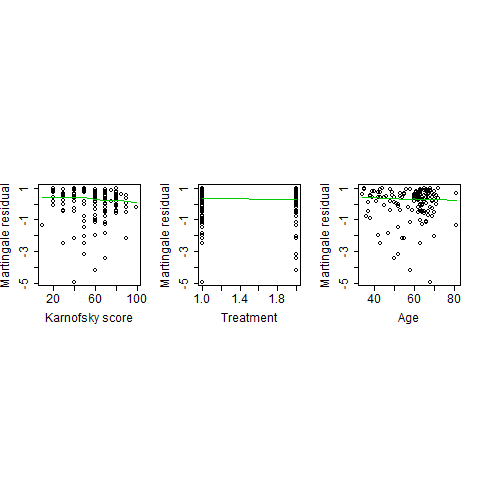
\includegraphics[width=0.95\textwidth, clip, trim={0 5cm 0cm 5cm}]{Figures/martingale_residuals.png}
\vskip100pt
\end{frame}


\begin{frame}
\frametitle{Deviance residuals}
\hspace*{-0.3in}
\begin{minipage}{0.12\textwidth}
\textcolor{white}{w}
\end{minipage}
\begin{minipage}{0.91\textwidth}
\small{
\begin{itemize}
\item[Use] Check for outliers, i.e. identify individuals whose outcome is poorly predicted
\item[Definition] Martingale residuals transformed to have mean 0 and roughly normal distribution
\item[Applies to] All subjects, for each predictor
\item[Interpretation] $>0$: subject $i$ experienced the event earlier than expected \\
                      $<0$: subject $i$ experienced the event later than expected
\item[Result] vector of length $n$ (\# of subjects)
\item[Plot] Plot subject IDs ($x$) versus deviance residuals ($y$) to determine which individuals should be screened.
\item[Check] Subjects with $|\mbox{deviance residuals}|>2.5$
\end{itemize}}
\end{minipage}
\end{frame}

\begin{frame}[fragile]
\frametitle{Deviance residuals in \texttt{R}}
\begin{Rcode}{0.0}
CR_mod <- coxph(Surv(time, status) ~ karno + trt + age,
                data = veteran)
veteran$deviance <- \textcolor{OrangeRed}{residuals}(CR_mod, type = \textcolor{OrangeRed}{"deviance"})

plot(x = 1:nrow(veteran),
     y = veteran$deviance,
     xlab = "Subject index",
     ylab = "Deviance residuals")
abline(h = 0)

veteran[abs(veteran$deviance) > 2.5, ]
\end{Rcode}
\end{frame}

\begin{frame}[fragile]
\frametitle{Deviance residual plots}
\begin{Rout}{-0.05}
   trt  celltype time status karno diagtime age prior  deviance
44   1 smallcell  392      1    40        4  68     0 -2.510903
73   2  squamous  231      0    50        8  52    10 -2.515511
85   2  squamous    1      1    50        7  35     0  2.566946
\end{Rout}
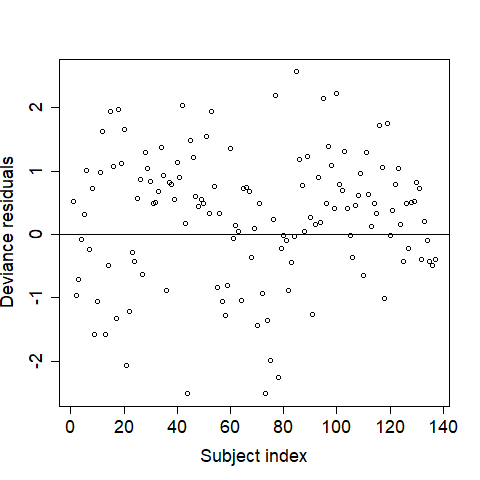
\includegraphics[width=0.45\textwidth, clip, trim={0 0cm 0cm 0cm}]{Figures/deviance_residuals.png}
\end{frame}


\begin{frame}
\frametitle{Schoenfeld residuals}
\hspace*{-0.3in}
\begin{minipage}{0.12\textwidth}
\textcolor{white}{w}
\end{minipage}
\begin{minipage}{0.91\textwidth}
\small{
\begin{itemize}
\item[Use] Identify violations of the proportional hazards assumption
\item[Definition] Difference between observed and expected predictor values (average value of the predictor at the subject's event time)
\item[Applies to] Only subjects with complete event times, for each predictor
\item[Interpretation] $>0$: subject $i$ has a larger predictor value than the event time suggests \\
                      $<0$: subject $i$ has a smaller predictor value than the event time suggests
\item[Result] $(m\times p)$ matrix; $m=$ complete event times, $p=$ \#predictors
\item[Plot] Plot the ordered \emph{complete} event times ($x$) versus the Schoenfeld residuals ($y$) for each predictor
\item[Check] Random pattern (flat smoothed curve) implies the proportional hazard (PH) assumption \emph{not} violated; otherwise, PH violated.
\end{itemize}}
\end{minipage}
\end{frame}

\begin{frame}[fragile]
\frametitle{Schoenfeld  residuals in \texttt{R}}
\begin{Rcode}{-0.06}
schoen <- \textcolor{OrangeRed}{residuals}(CR_mod, type = \textcolor{OrangeRed}{"schoenfeld"})
complete_times <- sort(veteran$time[veteran$status!=0])

par(mfrow = c(1,3), pty = "s")
plot(x = complete_times, y = schoen[,1], main = "Karnofsky score",
     xlab = "Complete times", ylab = "Schoenfeld residuals")
lines(lowess(complete_times, schoen[,1]), col = 3)

plot(x = complete_times, y = schoen[,2], main = "Treatment",
     xlab = "Complete times", ylab = "Schoenfeld residuals")
lines(lowess(complete_times, schoen[,2]), col = 3)

plot(x = complete_times, y = schoen[,3], main = "Age",
     xlab = "Complete times", ylab = "Schoenfeld residuals")
lines(lowess(complete_times, schoen[,3]), col = 3)
\end{Rcode}
\end{frame}

\begin{frame}[fragile]
\frametitle{Schoenfeld residual plots}
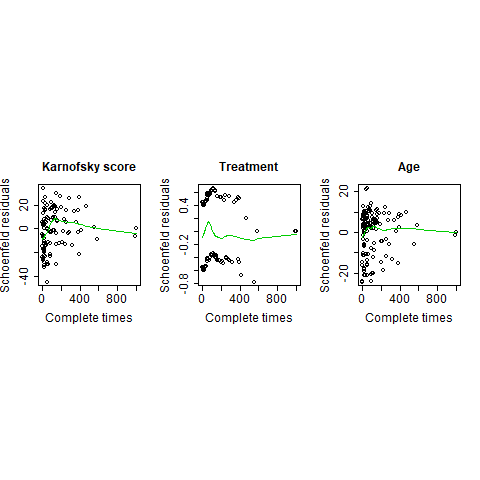
\includegraphics[width=0.95\textwidth, clip, trim={0 5cm 0cm 5cm}]{Figures/schoen_residuals.png}
\vskip100pt
\end{frame}




\begin{frame}
\frametitle{Formal test for PH assumption}
\begin{itemize}
\item It has been proposed (Grambsch and Therneau, 1994) that we can assume that $\beta$ depends on a
function of time $t$ by the relationship:
\begin{eqnarray}
\beta_j(t)=\beta_j+\gamma_jg_j(t),\nonumber
\end{eqnarray}
where $g$ is a specified function of time.  A commonly used function is $g(t)=\ln(t)$.
\item Under this model, we test whether $\gamma_j$ is significantly different from 0, i.e:
\item[] $H_0$: $\gamma_j = 0$ vs $H_a$: $\gamma_j \neq 0$
\item Failing to reject $H_0$ implies:
\item[] \emph{The PH assumption for $x_j$ has not been violated.}
\item Rejecting $H_0$ implies:
\item[] \emph{The PH assumption for $x_j$ has been violated.}
\end{itemize}
\end{frame}

\begin{frame}[fragile]
\frametitle{Formal test for PH assumption, in \texttt{R}}
\begin{Rcode}{0.0}
CR_mod <- coxph(Surv(time, status) ~ karno + trt + age,
                data = veteran)
\textcolor{OrangeRed}{cox.zph}(CR_mod, transform = "log")
\end{Rcode}
\begin{Rout}{0.45}
           rho chisq        p
\textcolor{OrangeRed}{karno   0.3154 12.13 0.000497}
trt    -0.0954  1.22 0.270034
\textcolor{OrangeRed}{age     0.2121  6.58 0.010308}
GLOBAL      NA 15.66 0.001334
\end{Rout}
\end{frame}

\begin{frame}
\frametitle{Score residuals}
\hspace*{-0.3in}
\begin{minipage}{0.12\textwidth}
\textcolor{white}{w}
\end{minipage}
\begin{minipage}{0.91\textwidth}
\small{
\begin{itemize}
\item[Use] Detecting overly influential observations
\item[Definition] A function of the approximate change in the parameter estimate that would result if the $i^{th}$ subject were removed from the sample.
\item[Applies to] All subjects, for each predictor
\item[Interpretation] $>0$: parameter estimate ($\hat{\beta}_j$) would increase without individual $i$ \\
                      $<0$: parameter estimate ($\hat{\beta}_j$) would decrease without individual $i$
\item[Result] $(n\times p)$ matrix; $n=$ \# subjects, $p=$ \#predictors
\item[Plot] Plot subject index ($x$) versus the score residuals ($y$) for each predictor.
\item[Check] Subjects with ``large" (in magnitude) score residuals are more influential on fit (no rule of thumb).
\end{itemize}}
\end{minipage}
\end{frame}


\begin{frame}[fragile]
\frametitle{Score  residuals in \texttt{R}}
\begin{Rcode}{-0.06}
score <- \textcolor{OrangeRed}{residuals}(CR_mod, type = \textcolor{OrangeRed}{"score"})

veteran[score[,1] > 100 |
        score[,1] < -50 |
        abs(score[,2]) > 2 |
        abs(score[,3]) > 40, ]

plot(x = 1:nrow(veteran),
     y = score[,1],
     xlab = "Subject index",
     ylab = "Score residuals",
     main = "Karnofsky score")
\end{Rcode}
\end{frame}

\begin{frame}[fragile]
\frametitle{Score residual plots}
\begin{Rout}{-0.05}
   trt  celltype time status karno diagtime age prior
44   1 smallcell  392      1    40        4  68     0
70   2  squamous  999      1    90       12  54    10
78   2  squamous  587      1    60        3  58     0
\end{Rout}
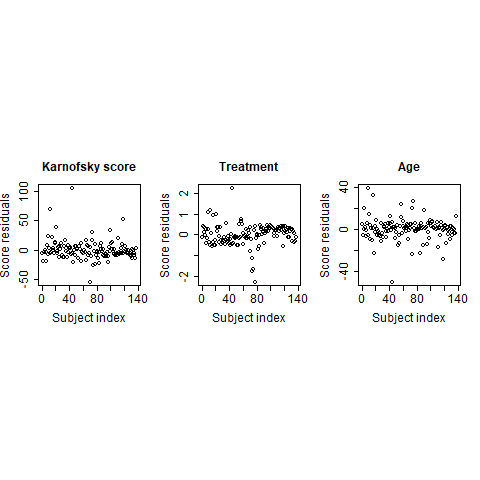
\includegraphics[width=0.95\textwidth, clip, trim={0 5cm 0cm 5cm}]{Figures/score_residuals.png}
\end{frame}



%===========================================================================================================================
\section[Next steps]{Next steps}
%===========================================================================================================================
\subsection{}
\begin{frame}
\tableofcontents[currentsection, hideallsubsections]
\end{frame}


\begin{frame}
\frametitle{Addressing findings}
\begin{itemize}
\item If you have identified some outlying or influential subjects:
\begin{enumerate}
\item Re-fit the model without the subjects who are influential and/or considered outliers.
\item Carefully decide if these observations should be included or not.
\item[]
\end{enumerate}
\item If you found a violation in the proportionality assumption:
\begin{enumerate}
\item Fit a ``stratified" model which posits the existence of different baseline hazard functions.
\item Fit a model that includes an interaction term between the predictor and the time variable (or a function of time); we'll focus more on strategy \# 1.
\end{enumerate}
\end{itemize}
\end{frame}


\begin{frame}
\frametitle{Stratified Cox model}
\begin{itemize}
\item When one or more predictors does not satisfy the proportional hazards assumption, the standard CR model is not appropriate, since we can no longer assume an identical baseline hazard function, $h_0(t)$, for each individual.
\item To accommodate different baseline hazard functions, a \emph{stratified CR model} can be fit that allows separate baseline hazard functions (not necessarily known) for each value (stratum) of the \textit{stratification variable}.
\item Suppose the stratification variable has $s$ levels. The stratified CR model assumes a different baseline hazard function corresponding to each value of the stratification variable, i.e. the form of the model is:
\begin{eqnarray}
h_s(t|X_1,...X_p) = h_0g(t)\exp(\beta_1X_1+\cdots+\beta_1X_1) \nonumber
\end{eqnarray}
where $g=1,\ldots,s$ and $s=$ number of levels of stratification variable.
\end{itemize}
\end{frame}

\begin{frame}
\frametitle{Stratified Cox model, cont.}
\begin{itemize}
\item The interpretation of the (estimated) coefficients and (estimated) hazard ratios are made adjusting for the other variables in the model \textit{and} the stratification variable.

\item \textbf{Violating predictor $X$ is categorical:}
\item[]each stratum can correspond to a different value of the predictor, and the stratification variable is identical to $X$.

\item \textbf{Violating predictor $X$ is quantitative:}
\item[] create a stratification variable by dividing $X$ into appropriate ranges, with each range corresponding to a stratum.

\item \textbf{Several violating predictors $X_1, \ldots,X_k$:}
\item[] then a stratification variable can be created based on combinations of $X_1, \ldots,X_k$.
\end{itemize}
\end{frame}

\begin{frame}[fragile]
\frametitle{Stratified Cox model in \texttt{R}}
\begin{Rcode}{0.0}
CR_mod_stratified <-
    coxph(Surv(time, status) ~ karno + \textcolor{OrangeRed}{strata(trt)} + age,
          data = veteran)
summary(CR_mod_stratified)
\end{Rcode}
\end{frame}

\begin{frame}[fragile]
\frametitle{Stratified Cox model in \texttt{R}}
\begin{Rout}{-0.05}
Call:
coxph(formula = Surv(time, status) ~ karno + strata(trt) + age,
    data = veteran)

  n= 137, number of events= 128

           coef exp(coef)  se(coef)      z Pr(>|z|)
karno -0.034227  0.966352  0.005417 -6.319 2.64e-10 ***
age   -0.003383  0.996622  0.009203 -0.368    0.713
---
Signif. codes:  0 ‘***’ 0.001 ‘**’ 0.01 ‘*’ 0.05 ‘.’ 0.1 ‘ ’ 1

      exp(coef) exp(-coef) lower .95 upper .95
karno    0.9664      1.035    0.9561    0.9767
age      0.9966      1.003    0.9788    1.0148
\end{Rout}
\end{frame}

\begin{frame}[fragile]
\frametitle{Stratified Cox model, interpretations}
\begin{itemize}
\item Even though you do not see \texttt{trt} in the \texttt{R} output, it is not being ignored!  It is taken into account in the baseline hazard function.
\item The hazard of death is estimated to decrease b 3.4\% for a 1 point increase in Karnofsky score, adjusting for age and treatment.
\item The estimated predictor adjusted survival curves are:
\begin{itemize}
\item[test trt:] $\displaystyle \left[\hat{S}_{01(t)} \right]^{\exp\left(-0.034X_1-0.003X_2 \right)}$
\item[standard trt:] $\displaystyle \left[\hat{S}_{02(t)} \right]^{\exp\left(-0.034X_1-0.003X_2 \right)}$
\end{itemize}
\end{itemize}
\end{frame}

\begin{frame}
\frametitle{Estimated stratified predictor-adjusted survival curves}
\begin{minipage}{0.60\textwidth}
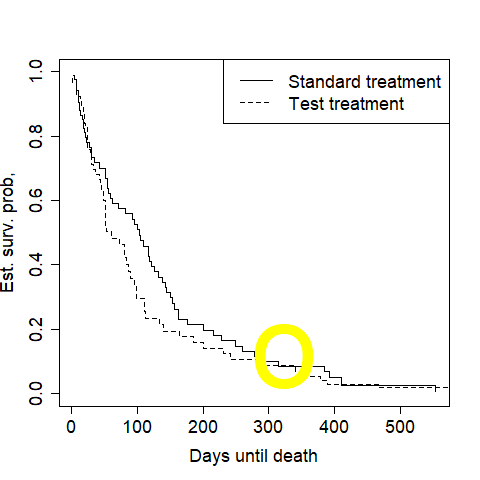
\includegraphics[width=1.0\textwidth, clip, trim={0 0cm 0cm 0cm}]{Figures/stratified_cox.png}
\end{minipage}
\blankcolumn
\begin{minipage}{0.30\textwidth}
Estimated survival curves now cross!
\end{minipage}
\end{frame}

\end{document}